%------------------
% General Settings
%------------------
\def \docTitle      {User Manual}
\def \docSubTitle   {SMC2242/SMC4242}
\def \productNumber {SMCx242}
\def \productName   {Stepper Motor Controller}
\def \docAuthor     {LK-Instruments}
\def \docSubject    {\docAuthor \docTitle \docSubTitle}
\def \docKeywords   {LK-Instruments, Stepper Motor Controller, SMC2242, SMC4242}

%\documentclass[a4paper, final, 12pt, twoside]{scrartcl}
\documentclass[a4paper, final, 12pt, oneside]{refart}

%----------
% Packages
%----------
\usepackage{etex}
\reserveinserts{30}
\usepackage[utf8]{inputenc}
%\usepackage[latin1]{inputenc} % erlaubt Umlaute in der tex-Datei

\usepackage{lmodern}                     % Latin Modern as Typewriter Font
\usepackage{slantsc}
\usepackage[urw-garamond]{mathdesign}
\usepackage{garamondx}
\usepackage[sfdefault]{sourcesanspro}    % SourceSan­sPro als serifenlose Schrift
\usepackage[T1]{fontenc}

\usepackage[english]{babel}              % For the hyphenations in different languages
\usepackage[intlimits]{amsmath}          % math symbols
\usepackage{braket}                      % Dirac braket notation
\usepackage{graphicx}                    % include pictures
\usepackage{color}
%\usepackage[shell]{gnuplottex}           % gnuplot in latex
\usepackage{pstricks}                    % post script tricks
\usepackage{listings}                    % enter programming code
\usepackage{fancyhdr}                    % make quite nice header/footer
%\usepackage[version=3]{mhchem}           % chemistry stuff
\usepackage{relsize}
\usepackage{afterpage}
\usepackage{gensymb}
\usepackage{textcomp}
\usepackage{listings}					 % erlaubt Quellcode mit Zeilenumbruechen

\usepackage{makeidx}                     % create index
  \makeindex
\usepackage[totoc]{idxlayout}            % index in contents
  
\usepackage{lcd}						 % Character LCD
%\usepackage[paperheight=210mm,paperwidth=210mm,margin=20mm,heightrounded]{geometry}
\usepackage{multirow}
\usepackage{booktabs}
\usepackage{colortbl}
\usepackage{tabularx}


\usepackage{pgfplots}
\usepackage{tikz}                        % beautiful plots
\pgfplotsset{compat = newest}
\usepackage{units}                       % easy to use number-unit-package
\usepackage[section]{placeins}           % Float barrier for sections.

\usepackage{float}                       % lädt das Paket zum erzwingen der Grafikposition
\usepackage{morefloats} 

\usetikzlibrary{shapes.geometric, arrows}	% Flow chart

\newfont{\ce}{cerm}                      
\def\CE#1{{\font\ce=#1\ce CE}}


%----------------
% PDF properties
%----------------
\usepackage[
  pdftitle={\docAuthor~\docSubTitle~\docTitle}
 ,pdfsubject={\docSubject}
 ,pdfauthor={\docAuthor}
 ,pdfkeywords={\docKeywords}
 ,pdfcreator={\docAuthor}
 ,pdfstartview=Fit                       % startseite ganz anzeigen
 ,pdfborder={0 0 0}                      % links ohne umrandungen
 ,pdfdisplaydoctitle=true                % pdftitle statt dateinamen anzeigen
 ,pdfcenterwindow=true                   % position pdf in center of the screen
 ,setpagesize=true
]{hyperref}

%-------------------
% Header und Footer
%-------------------
\pagestyle{fancy}
\fancyhf{}        % clear all header/footer
\renewcommand{\headrulewidth}{0pt}
\renewcommand{\sectionmark}[1]{\markboth{#1}{}}
\renewcommand{\subsectionmark}[1]{\markright{#1}}
\fancyhead[LE,RO]{\textbf{\thepage}}
\fancyhead[CE]{\footnotesize{\textit{\nouppercase{\rightmark}}}}
\fancyhead[CO]{\footnotesize{\scshape{\nouppercase{\leftmark}}}}

% number equations with sections before equation-index
\numberwithin{equation}{section}
\numberwithin{table}{section}
\numberwithin{figure}{section}

%---------------------
% My code definitions
%---------------------

\newtheorem{envdefinition}{Definition}[section]
\newtheorem{envsatz}{Satz}

% special numbers and letters
\renewcommand{\i}{\mathrm{i}}                  % complex i
\newcommand{\e}{\mathrm{e}}                    % Eulers number
\renewcommand{\phi}{\varphi}                   % nicer phi
\renewcommand{\epsilon}{\varepsilon}           % nicer epsilon
\renewcommand{\theta}{\vartheta}               % nicer theta
\renewcommand{\rho}{\varrho}                   % nicer rho
%\newcommand{\degree}{^{\circ}}                 % degree-circle

% vectors and matrices
\renewcommand{\vec}[1]{\boldsymbol{#1}}
\newcommand{\Vek}[3]{\left(\begin{array}{c}#1\\#2 
\ifthenelse{\equal{#3}{}}{}{\\#3}\end{array}\right)}

% integral and derivative stuff:
\renewcommand{\d}[1]{\;\mathrm{d}#1}           % integeration d
% total derivative
\newcommand{\td}[1]{\frac{\mathrm{d}}{\mathrm{d}#1}\,}
\newcommand{\pd}[1]{\partial_{#1}\,}             % partial derivative

% Braket notation
\renewcommand{\bra}{\Bra}
\renewcommand{\ket}{\Ket}
\renewcommand{\braket}{\Braket}
\renewcommand{\set}{\Set}

% plus-minus with braces
\newcommand{\PM}{\ensuremath{\substack{+\\[-0.25em]-}\,}}
\renewcommand{\pm}{\PM}
\newcommand{\pmp}{\ensuremath{\substack{\mathsmaller{(}+\mathsmaller{)}\\[-0.25em]-}\,}}
\newcommand{\pmm}{\ensuremath{\substack{+\\[-0.25em]\mathsmaller{(}-\mathsmaller{)}}\,}}

%---------------------
% LCD
%---------------------

\definecolor{lightgrey}{rgb}{0.9,0.9,0.9}
\definecolor{darkgrey}{rgb}{0.2,0.2,0.2}
\definecolor{black}{rgb}{0,0,0}
\LCDcolors{black}{lightgrey}
\DefineLCDchar{degree}{11100101001110000000000000000000000}

%---------------------
% Index
%---------------------


%----------------------------------------------------------
% let the party start
%----------------------------------------------------------
\begin{document}

\thispagestyle{empty}

%
\pagecolor{black}
.
\vspace{4cm}
\begin{center}
  \includegraphics[width=0.6\textwidth]{../general/logo_white.pdf}
\end{center}

\vspace*{2cm}
\begin{center}
  {\color{white} \Huge\textbf{\textsf{\docTitle}}}
\end{center}

\vspace*{1cm}
\begin{center}
  {\color{white} \Huge\textbf{\textsf{\productName}}}
\end{center}

%\vspace*{0.5cm}
\begin{center}
  {\color{white} \Huge\textbf{\textsf{\docSubTitle}}}
\end{center}

\afterpage{\nopagecolor}
\newpage


%\pagecolor{black}
.
\vspace{4cm}
\begin{center}
  
\includegraphics[width=0.6\textwidth]{../general/logo_black.pdf}
\end{center}

\vspace*{2cm}
\begin{center}
  {\Huge\textbf{\textsf{\docTitle}}}
\end{center}

\vspace*{1cm}
\begin{center}
  {\Huge\textbf{\textsf{\productName}}}
\end{center}

%\vspace*{0.5cm}
\begin{center}
  {\Huge\textbf{\textsf{\docSubTitle}}}
\end{center}

\afterpage{\nopagecolor}
\newpage

\clearpage

% to get an empty page
\newpage\null
\thispagestyle{empty}
\newpage


%\thispagestyle{empty}
\section*{Notices}
\sectionmark{Notices}
\textcopyright~\docAuthor~2016.
No part of this manual may be reproduced in any form or by any means
(including electronic storage and retrieval or translation into a
foreign language) without prior agreement and written consent from \docAuthor.

\subsection*{Edition}
\today

\subsection*{Warranty}
The material contained in this document is provided \glqq as is\grqq, and is subject to
being changed, without notice, in future editions. Further, to the maximum extent
permitted by applicable law, \docAuthor~disclaims all warranties, either express or
implied, with regard to this manual and any information contained herein,
including but not limited to the implied warranties of merchantability and fitness
for a particular purpose.

\docAuthor~ shall not be liable for errors or for incidental
or consequential damages in connection with the furnishing, use, or performance of
this document or of any information contained herein. Should \docAuthor~and
the user have a separate written agreement with warranty terms covering the material
in this document that conflict with these terms, the warranty terms in the
separate agreement shall control.

\subsection*{Technology Licenses}
The hardware and/or software described in this document are furnished under a
license and may be used or copied only in accordance with the terms of such license.

%\subsection*{Restricted Rights Legend}
%If software is for use in the performance of a U.S. Government prime contract or
%subcontract, Software is delivered and licensed as “Commercial computer software”
%as defined in DFAR 252.227-7014 (June 1995), or as a “commercial item” as defined
%in FAR 2.101(a) or as “Restricted computer software” as defined in FAR 52.227-19
%(June 1987) or any equivalent agency regulation or contract clause. Use,
%duplication or disclosure of Software is subject to BitifEye’s standard commercial
%license terms, and non-DOD Departments and Agencies of the U.S. Government will
%receive no greater than Restricted Rights as defined in FAR 52.227-19(c)(1-2)
%(June 1987). U.S. Government users will receive no greater than Limited Rights as
%defined in FAR 52.227-14 (June 1987) or DFAR 252.227-7015 (b)(2) (November 1995),
%as applicable in any technical data.

%\subsection*{Safety Notices}


%\subsection*{Product Labels}
%\begin{itemize}
%  \item[\CE{cerm scaled \magstep5}] This electronic product is in compliance
%                                    with the EMC and Safety regulations of
%                                    the European Community.
%\end{itemize}



\newpage

\section{Technical Assistance}
If you need product assistance or if you have suggestions, contact \docAuthor.
You will find the contact information on the \docAuthor~homepage at
\begin{center}
  \url{http://www.lk-instruments.com}
\end{center}
Representatives of \docAuthor~are available during standard German business hours.
Before you contact \docAuthor, please note the actions you took before you experienced
the problem. Then describe those actions and the problem to the technical support
engineer.

\subsection{Found a mistake?}
We encourage comments about this publication. Please report any mistakes
to \docAuthor:
\begin{center}
  \href{mailto:support@lk-instruments.com}{\nolinkurl{support@lk-instruments.com}}
\end{center}






\newpage
\clearpage

\pagenumbering{roman}   % small roman page numbering

\tableofcontents
\newpage

\listoffigures
\listoftables

% to get an empty page
\newpage\null
\thispagestyle{empty}
\newpage

\pagenumbering{arabic}  % now arabic page numbering
                        % for the rest of the document
\newpage

Thank you for purchasing the \productNumber ~\productName. This user
manual will explain you how to operate the \productName. Please take
some time to read it carefully before operating the device. Keep the
instructions in a safe place for future reference.

\section{Introduction}
The \productNumber ~\productName ~is a universal controller for  bipolar stepper motors. It can be used to drive two (SMC2242) or four (SMC4242) stepper motors.
% There are three different firmware version available SMCx242-R for rotary axis, SMCx242-L for linear motion and SMCx242-U which features both options.
It is designed to work perfectly together with  our assortment of stepper motor driven stages, but it might be also used to drive 3\textsuperscript{rd} party motors or stages.

\subsection{Package contents}
Please check that the package contains all the following items:
\begin{itemize}
\item \productNumber ~\productName
%\item Power supply
\item USB cable
\item User Manual
\end{itemize}

\subsection{Installing the device}
The \productName ~is designed for the inside use. Therefore it should not be used outside and kept away from water and moisture. Do not operate the unit near any heat sources or in direct sun light. When installing the device ensure to put it on a flat and leveled surface. Also ensure that there is adequate space around the device for ventilation.\\
After moving the unit to a different location, condensation inside the unit may occur. In this case please wait for some hours before you connect the \productName ~to the power supply.\\
Connect the device only to power sources that meet the specifications written on its rear panel.

\begin{figure}[h]
  \centering
  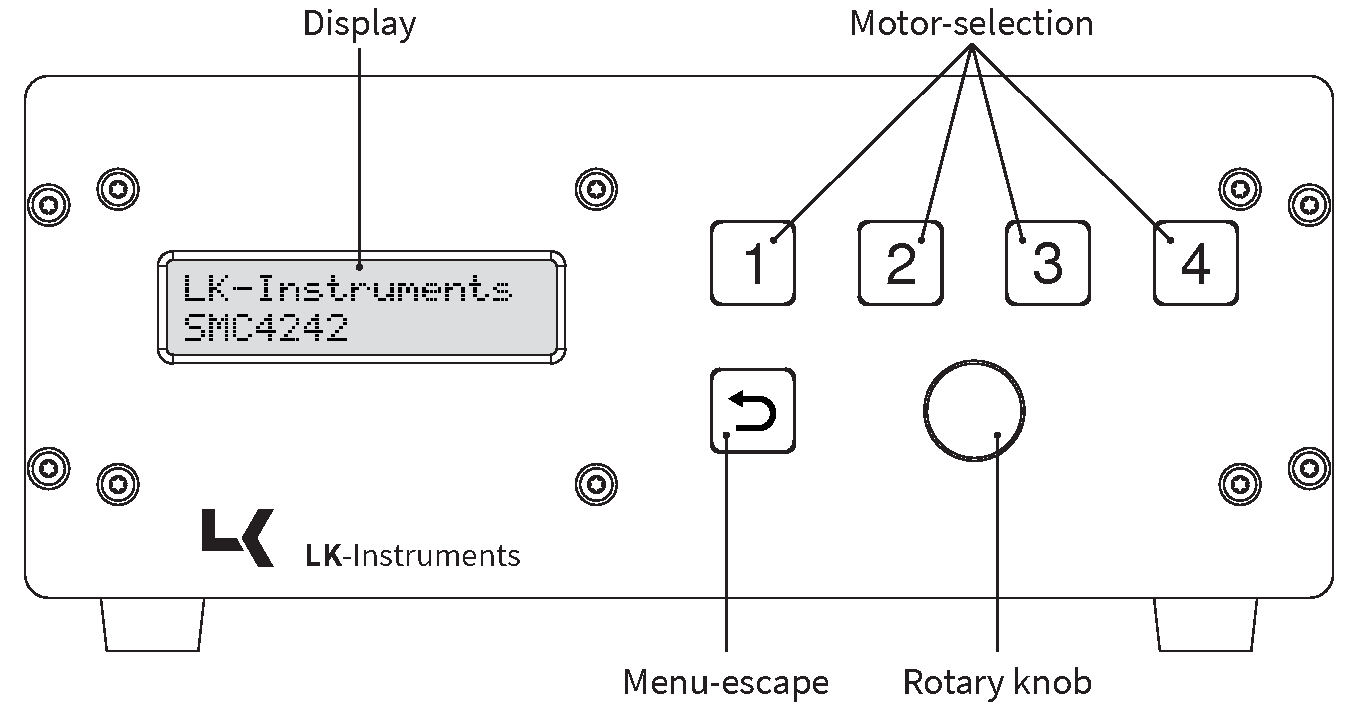
\includegraphics[angle=0,origin=c,width=1\textwidth]{./grafiken/MG22131_front_text_2.pdf}
  \caption[Front view of \productNumber .]{Front view of the \productNumber ~\productName .}
  \label{frontpanel}
\end{figure}

\begin{figure}[h]
  \centering
  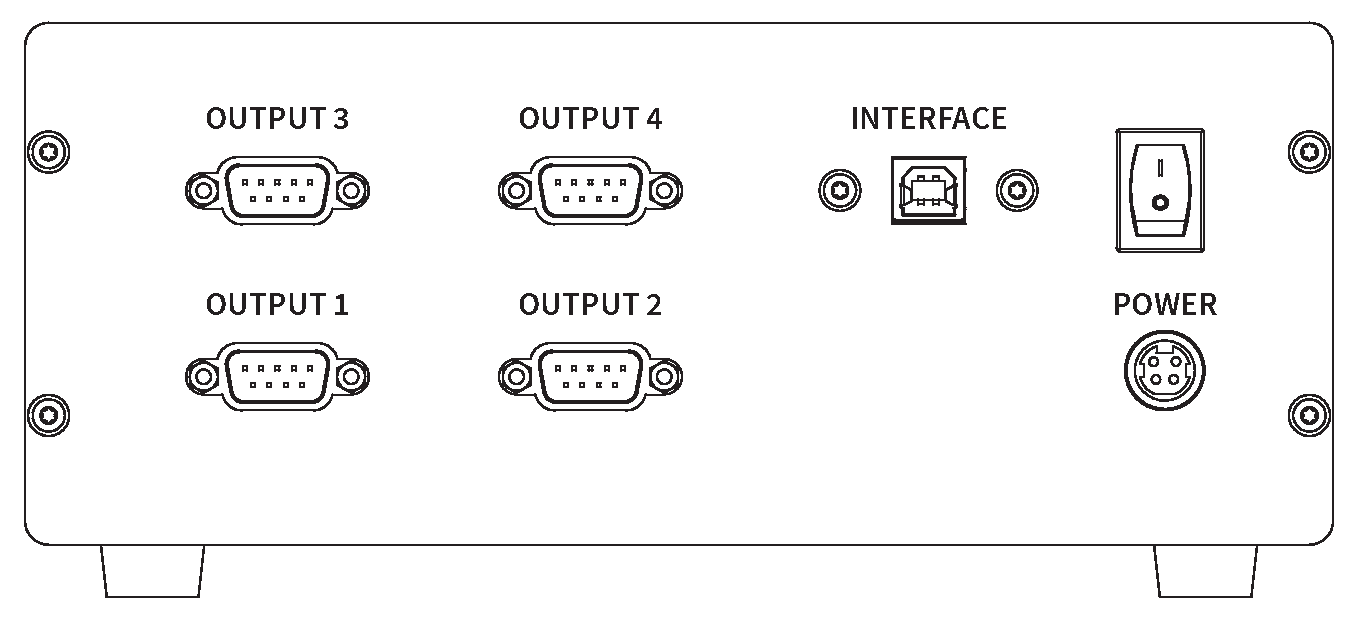
\includegraphics[angle=0,origin=c,width=1\textwidth]{./grafiken/MG22131_back_text.pdf}
  \caption[Rear view of \productNumber .]{Rear view of the \productNumber ~\productName .}
  \label{frontpanel}
\end{figure}



%\newpage
\clearpage
\section{General Operation}
\label{chp:general_operation}
The \productNumber ~\productName ~features two operation modes. It can be
either operated using the manual user interface or remote controlled by a
computer. In this section the manual operation of the device is explained.

After turning on the \productName ~it comes up with its start screen.
Turning the rotary knob serves to scroll through the menus (see
figure~\ref{main_menu}). Pressing the rotary knob enters the selected
menu. Pressing the menu-escape-button leaves the menu again.

\subsection{Display structure}
In almost every menu four values are displayed. Depending on the previously
selected menu the values correspond to different quantities. Where
\begin{itemize}
  \item the upper left value accompanies to Motor 1
  \item the upper right value accompanies to Motor 2
  \item the lower left value accompanies to Motor 3
  \item the lower right value accompanies to Motor 4
\end{itemize}

\subsection{Motor selection}
To select a motor there are four buttons. Motor selection can solely be done in an entered menu. To select a motor, press the respective motor-selection button. A selected motor is signed with an arrow on the display and by a color change of the corresponding motor-selection button. Pressing the selection-button again deselects the motor. Once a motor is selected its appropriate value can be changed by turning the rotary knob. If multiple motors are selected at the same time, there values will be changed simultaneously. By leaving a menu without motor deselection the selected motor(s) stay selected in any other menu.

\tikzstyle{menu_style} = [rectangle, rounded corners, minimum width=3cm, minimum height=1cm,text centered, draw=black]
\tikzstyle{arrow} = [thick,<->,>=latex]
\def \textWidth {5cm}

\begin{figure}[H]
\begin{tikzpicture}[node distance=2cm]
\node (start) [menu_style] {
\begin{minipage}[h]{5cm}
\LCD{2}{16}|LK-Instruments|
|SMC4242|
\end{minipage}
 \hfill
\begin{minipage}[h]{\textWidth}
Start screen\\
Display firmware version.
\end{minipage}
};

\node (motor_pos) [menu_style, below of=start] {
\begin{minipage}[h]{5cm}
\LCD{2}{16}|Change motor|
|position|
\end{minipage}
 \hfill
\begin{minipage}[h]{\textWidth}
%Change motor position:\\
Position is displayed and can be changed.
\end{minipage}
};

\node (step_multiplier) [menu_style, below of=motor_pos] {
\begin{minipage}[h]{5cm}
\LCD{2}{16}|Set step|
|multiplier|
\end{minipage}
 \hfill
\begin{minipage}[h]{\textWidth}
%Set step multiplier\\
Edit multiplier for rotary knob.
\end{minipage}
};

\node (step_unit) [menu_style, below of=step_multiplier] {
\begin{minipage}[h]{5cm}
\LCD{2}{16}|Change step|
|unit|
\end{minipage}
 \hfill
\begin{minipage}[h]{\textWidth}
%Menu: Change step unit\\
Define the displayed unit.
\end{minipage}
};

\node (internal_prog) [menu_style, below of=step_unit] {
\begin{minipage}[h]{5cm}
\LCD{2}{16}|Run internal|
|program|
\end{minipage}
 \hfill
\begin{minipage}[h]{\textWidth}
%Menu: Run internal program\\
Step through the program list.
\end{minipage}
};

\node (const_speed) [menu_style, below of=internal_prog] {
\begin{minipage}[h]{5cm}
\LCD{2}{16}|Run with|
|constant speed|
\end{minipage}
 \hfill
\begin{minipage}[h]{\textWidth}
%Menu: Set constant angular speed\\
Start/Stop continuous\\ movement.
\end{minipage}
};

\node (optical_zero) [menu_style, below of=const_speed] {
\begin{minipage}[h]{5cm}
\LCD{2}{16}|Define zero|
|position|
\end{minipage}
 \hfill
\begin{minipage}[h]{\textWidth}
%Menu: Define optical zero position\\
Edit the zero offset.
\end{minipage}
};

\node (zero_cal) [menu_style, below of=optical_zero] {
\begin{minipage}[h]{5cm}
\LCD{2}{16}|Run zero|
|calibration|
\end{minipage}
 \hfill
\begin{minipage}[h]{\textWidth}
%Menu: Run zero calibration\\
Find mechanical zero\\ position.
\end{minipage}
};

\node (settings) [menu_style, below of=zero_cal] {
\begin{minipage}[h]{5cm}
\LCD{2}{16}|Enter|
|settings menu|
\end{minipage}
 \hfill
\begin{minipage}[h]{\textWidth}
Enter the settings menu.
\end{minipage}
};



\draw [arrow] (start) -- (motor_pos);
\draw [arrow] (motor_pos) -- (step_multiplier);
\draw [arrow] (step_multiplier) -- (step_unit);
\draw [arrow] (step_unit) -- (internal_prog);
\draw [arrow] (internal_prog) -- (const_speed);
\draw [arrow] (const_speed) -- (optical_zero);
\draw [arrow] (optical_zero) -- (zero_cal);
\draw [arrow] (zero_cal) -- (settings);
\draw [arrow] (settings.east) -- +(1,0) |- (start.east);
\end{tikzpicture}
\caption[Overview of the available menus.]{Overview of the available menus. By turning
the rotary knob one can navigate through the menus as indicated by the arrows.}
\label{main_menu}
\end{figure}

\FloatBarrier



\subsection{Start screen}
By pressing the rotary knob while the start screen is active the
firmware version will be displayed.
\begin{center}
  \LCD{2}{16}|SMCx242|
             |Firmware 1.5|
\end{center}
Firmware updates are available at \url{http://www.lk-instruments.com} on
the corresponding product website.

%\begin{macrocode}
%\DefineLCDchar{degree}{11100101001110000000000000000000000}
%\end{macrocode}

\subsection{Motor position}
\label{menu_motor_pos}
\index{change!position}
This menu displays the current motor positions and allows them to be changed. The default display unit is degree, which can be changed to the users preferred unit, see \ref{chp:change_step_unit}. The position of a selected motor can be changed by turning the rotary knob.\\
Default steps for the available units are:
\begin{itemize}
\item $1\degree$ if unit is degree
\item $\frac{\pi}{8}$ if unit is radian
\item 1 step if unit is steps
\end{itemize}
\begin{center}
  \LCD{2}{16}|{rarrow}0.0{pi}   {rarrow}0.0{degree} |
             |{rarrow}0st    {rarrow}0.0{degree} |
\end{center}


\paragraph{Fast moving mode}
\index{fast moving mode}
When pressing the rotary knob inside the change-motor-position-menu one enters the fast moving mode. Pressing the rotary knob again disables the fast moving mode. The fast moving mode is indicated by another marking arrow for the corresponding motor.\\
%The fast moving mode will only be enabled or disabled for selected motors.
Default steps in this mode are:
\begin{itemize}
  \item $10\degree$ if unit is degree
  \item $\frac{\pi}{8}$ if unit is radian
  \item 100 steps if unit is steps
\end{itemize}
The snapped display shows the different indicating arrows.
\begin{center}
  \LCD{2}{16}|>10.0{degree} >0.0{degree} |
             |>0.0{degree}  >0.0{degree} |
\end{center}


\subsection{Step multiplier}
\index{step multiplier}
In this menu the step multipliers can be adjusted. If the step multiplier differs from 1.0 the corresponding motor will rotate more or less steps with each click of the rotary knob. It is also possible to turn the motors in different directions by applying a negative step multiplier to a motor. A step multiplier can only be applied if the step unit is degree or radians. The factory default value for all motors is 1.0.\\
Example: If the step multiplier for motor 1 is 1.0, the step multiplier for motor 2 is 4.0 and the step multiplier for motor 3 is -2.0, when changing the motors positions motor 2 will move four times more steps than motor 1 and motor 3 will move twice as many steps as motor 1, but in the opposite direction. 
%Negative values are allowed as well. This will result in counter direction movements.
\begin{center}
  \LCD{2}{16}|{rarrow}1.0x   {rarrow}4.0x|
             |{rarrow}-2.0x   1.0x|
\end{center}

\subsection{Step unit}
\label{chp:change_step_unit}
\index{change!unit}
In this menu one can choose the unit of the displayed position. Note, that changing the unit will also affect the step width, see~\ref{menu_motor_pos}. There are three possible choices for each motor:
\begin{itemize}
\item degree
\item radian
\item step
\end{itemize}
\begin{center}
  \LCD{2}{16}|{rarrow}radian {rarrow}degree|
             |{rarrow}step    degree|
\end{center}

\subsection{Internal program}
\index{internal program}
This menu allows the user to step through the internal program list with the rotary knob.
This function is only available if a program has previously been defined (see \ref{section_instruction_set}).
Internal programs are also saved to the device when the current configuration is saved, see \ref{menu_save}.
\begin{center}
  \LCD{2}{16}|Program running|
             |Step 0|
\end{center}

\subsection{Constant movement}
Here the motors can be set into an infinite moving state in clockwise (CW) or counter clockwise (CCW) direction. To get the motors moving with different velocities one needs to change the wait times between two steps (see \ref{menu_step_wait_time}).
STOP means that the motor is not moving. Constant speed for a certain motor can not be activated if a forbidden zone is configured for this motor (see \ref{chp:forbidden_zone}).
\begin{center}
  \LCD{2}{16}|{rarrow}CW     {rarrow}CCW|
             | STOP    STOP|
\end{center}

\subsection{Zero position}
\index{zero!position}
In this menu one can define an offset for the zero position. This is necessary due to a mostly unknown placement of the load mounted to a stage. 
%Here one can once adjust the desired optical zero position manually. 
The zero position is always defined in steps. In this menu there is also a fast mode available (please refer to  \ref{menu_motor_pos} for details about the fast mode). After adjustment it is recommended to save this configuration (see \ref{menu_save}). When performing a zero calibration, as explained in \ref{menu_zero_cal}, the zero position will have the defined offset form the mechanical zero position.
\begin{center}
  \LCD{2}{16}|{rarrow}122st   0st|
             | 0st     0st|
\end{center}

\subsection{Zero calibration}
\label{menu_zero_cal}
\index{zero!calibration}
Here one can calibrate the motor zero position for each motor. To perform a zero calibration select the motors to be calibrated and turn the rotary knob. Note, that during zero calibration no actions can be done on the device, even serial commands will not be accepted. The zero calibration will automatically deselect a motor when its calibration is finished. The zero calibration menu will be automatically leaved when calibration is finished.
\begin{center}
  \LCD{2}{16}|{rarrow}Mot 1  {rarrow}Mot 2|
             | Mot 3   Mot 4|
\end{center}

\subsection{Settings menu}
\label{menu_settings}
\index{settings}
The settings menu contains several submenus that allow the user to adjust some of the settings.\\
Turning the rotary knob serves to scroll through the settings menus (see figure~\ref{settings_menu}). Pressing the rotary knob enters the selected settings menu. Pressing the menu-escape-button leaves the settings menu.

\begin{figure}[H]
\begin{tikzpicture}[node distance=2cm]
\node (substep) [menu_style] {
\begin{minipage}[h]{5cm}
\LCD{2}{16}|Change motor|
|substep|
\end{minipage}
 \hfill
\begin{minipage}[h]{\textWidth}
%Menu: Change motor substep\\
Edit number of substeps\\ used for microstepping.
\end{minipage}
};

\node (motor_curr) [menu_style, below of=substep] {
\begin{minipage}[h]{5cm}
\LCD{2}{16}|Change motor|
|current|
\end{minipage}
 \hfill
\begin{minipage}[h]{\textWidth}
Adjust the maximum motor current.
\end{minipage}
};

\node (step_wait_time) [menu_style, below of=motor_curr] {
\begin{minipage}[h]{5cm}
\LCD{2}{16}|Change step|
|wait time|
\end{minipage}
 \hfill
\begin{minipage}[h]{\textWidth}
%Menu: Change step wait time\\
Edit time between steps.
\end{minipage}
};

\node (save) [menu_style, below of=step_wait_time] {
\begin{minipage}[h]{5cm}
\LCD{2}{16}|Save current|
|configuration|
\end{minipage}
 \hfill
\begin{minipage}[h]{\textWidth}
%Menu: Save all current configurations\\
Save configuration to\\ EEPROM.
\end{minipage}
};

\node (load) [menu_style, below of=save] {
\begin{minipage}[h]{5cm}
\LCD{2}{16}|Load last|
|configuration|
\end{minipage}
 \hfill
\begin{minipage}[h]{\textWidth}
%Menu: Load last configuration\\
Load configuration from EEPROM.
\end{minipage}
};

\draw [arrow] (substep) -- (motor_curr);
\draw [arrow] (motor_curr) -- (step_wait_time);
\draw [arrow] (step_wait_time) -- (save);
\draw [arrow] (save) -- (load);
\draw [arrow] (load.east) -- +(1,0) |- (substep.east);
\end{tikzpicture}
\caption[Overview of the settings menus.]{Overview of the settings menus. By turning
the rotary knob one can navigate through the settings menus as indicated by the arrows.}
\label{settings_menu}
\end{figure}



\subsubsection{Motor substeps}
\label{menu_substeps}
\index{change!substeps}
\index{change!microstepping}
In this menu one can change the number of substeps used for microstepping. Possible values are 1, 2, 4, 8, 16 or 32.\\
Note, that a value of 1 is equivalent to full step operation. So no microstepping is used to drive the stepper motor. If the adjusted value differs from 1, microstepping is used to obtain finer positioning resolution. Values above 8 are not recommended because of the decreasing motor torque.
\begin{center}
  \LCD{2}{16}|{rarrow}1      {rarrow}2|
             | 4      {rarrow}8|
\end{center}

\paragraph{A note on microstepping.}
\index{microstepping}
When increasing the number of substeps (microsteps per full step) the incremental torque per microstep decreases heavily. The expression for calculating the incremental tourque $\tau_{\text{inc}}$ is
\begin{equation*}
  \tau_{\text{inc}} = \tau_{\text{H}} \cdot \sin \left( \frac{90}{\mu} \right),
\end{equation*}
where $\tau_{\text{H}}$ is the holding torque per full step (without microstepping) and $\mu$ is the number of microsteps per full step.\\
The incremental torque $\tau_{\text{N}}$ for $N$ microsteps is
\begin{equation*}
  \tau_{\text{N}} = \tau_{\text{H}} \cdot \sin \left( \frac{90\cdot N}{\mu} \right).
\end{equation*}
So, the holding torque per microstep decreases as shown in table \ref{tab:microstepping_holding_torque}.
\begin{table}
  \centering
  \begin{tabular}{cc}
    \toprule
    \textbf{Microsteps per full step} & \textbf{Holding torque per microstep} \\
    \toprule
    1 & 100 \% \\ \midrule
    2 & 70.7 \%\\ \midrule
    4 & 38.3 \% \\ \midrule
    8 & 19.5 \% \\ \midrule
    16 & 9.8 \% \\ \midrule
    32 & 4.9 \% \\
    \bottomrule
  \end{tabular}
  \caption{Decrease of motor holding torque in dependence of the number of adjusted microsteps.}
  \label{tab:microstepping_holding_torque}
\end{table}

\subsubsection{Motor current}
\label{menu_motor_current}
\index{change!current}
In this menu the user can change the maximum current that is used to drive the corresponding stepper motor. Please ensure, that the value set here does not exceed the maximum ratings of your motor. 
\begin{center}
  \LCD{2}{16}| 1.0 A  {rarrow}1.3 A|
             |{rarrow}0.9 A   0.5 A|
\end{center}

\subsubsection{Step wait time}
\label{menu_step_wait_time}
\index{change!step wait time}
Here the wait time between two steps can be changed. This results in faster or slower movements of the stepper motor. The default value is 3 milliseconds.\\
Note, that a very short wait time and therefore fast movement speed can lead to stalling of the stepper motor.
%We do not recommend to use shorter wait times as 3 milliseconds.
\begin{center}
  \LCD{2}{16}|{rarrow}3 ms   {rarrow}5 ms|
             |{rarrow}18 ms   3 ms|
\end{center}

\subsubsection{Save current configuration}
\label{menu_save}
\index{save}
To save the current \productName ~configuration enter this menu and turn the rotary knob in any direction.\\
%The menu will be automatically leaved when saving is finished.
Note, that always the configuration for all motors will be saved. It is not possible to save the configuration for a single motor only.
\begin{center}
  \LCD{2}{16}|Save all current|
             |configurations|
\end{center}


\subsubsection{Load configuration}
\label{chp:menu_load}
\index{load}
To load the last saved \productName ~configuration enter this menu and turn the rotary knob in any direction.\\
%The menu will be leaved automatically when loading has finished.
Note: The last saved configuration is loaded automatically when powering on or resetting the \productName.\\
Note: There is just one memory space for a configuration.
\begin{center}
  \LCD{2}{16}|Load all saved|
             |configurations|
\end{center}


%\subsection{Forbidden zones}
%\label{chp:forbidden_zone}

%\subsection{Positioning procedures}
%\label{chp:positioning_procedure}





%\newpage

\clearpage
\section{Basic setup}

\subsection{Stepper motor setup}
Before a stepper motor is connected to the \productName , please ensure, that the following parameters are set according to the specifications of you stepper motor.

\begin{itemize}
\item maximum motor current
\item current decay mode
\item gear ratio
\item steps per full rotation
\item number of substeps
\item wait time between steps
\end{itemize}

\textbf{Warning:} Take especially care, that the maximum motor current does not exceed the maximum ratings of your stepper motor. A high current might damage the stepper motor or the \productName .

The parameters can be set to the desired value either using the manual user interface (see chapter \ref{chp:general_operation}) or via remote control through a computer (see chapter \ref{chp:remote_programming}).

\subsection{Example setup for M101A}
In the following configuration example it is assumed, that four LK-Instruments M101A rotation stages shall be connected to the \productName . In case different stepper motors shall be connected to the \productName , the same procedure applies, but you need to take care to change the values according to the data sheet of the stepper motor used.

\subsubsection{Motor current}
Before any of the stepper motors or rotation stages are connected to the \productName ~the maximum motor current needs to be adjusted. In the data sheet of the M101A rotation stage a typical motor current of \unit[1.3]{A} is specified.\\
In order to adjust the settings of the \productNumber ~\productName ~to this value, connect it to an appropriate power source and turn it on using the switch on its back panel.

There are two possible ways of adjusting the current setting either using the manual user interface or via remote control.\\
To adjust the setting using the manual user interface, navigate to the settings menu by rotating the rotary knob until the settings menu shows up (see \ref{chp:general_operation}). Enter this menu by pressing the rotary knob and navigate to the motor current menu by rotating the rotary knob (see \ref{menu_settings}). Enter the current menu by pressing the rotary knob (see \ref{menu_motor_current}). Now select all motors by pressing the corresponding motor-selection buttons and adjust the the motor current to the desired value of \unit[1.3]{A} by turning the rotary knob.\\
The next step is to save the settings to the EEPROM. To do so, exit the current menu by pressing the menu-escape-button once. Navigate to the save current configuration menu and enter it by pressing the rotary knob (see \ref{menu_save}). To save the configuration turn the rotary knob in any direction. If successful the word "saved" will show up on the display.

To adjust the settings using the remote interface, connect the \productName ~to a free USB port of a computer and connect to it, as described in chapter \ref{chp:remote_programming}, using a serial terminal. To set the motor current of all four motors to \unit[1.3]{A} and save the settings to the EEPROM issue the following commands:

\texttt{SETCURR 0 1.3}\\
\texttt{SETCURR 1 1.3}\\
\texttt{SETCURR 2 1.3}\\
\texttt{SETCURR 3 1.3}\\
\texttt{SAVECONF}

Now one may already connect the stepper motors to the \productName . To do so, first turn of the \productName , connect the stepper motors to its outputs and once connected, turn it back on.

\subsubsection{Current decay mode}
The \productNumber ~\productName ~allows the user to select between three different current decay modes, namely fast, slow and mixed decay. In this example we would like to set to decay mode to slow. Therefore the following commands need to be send:

\texttt{SETDECAY 0 0}\\
\texttt{SETDECAY 1 0}\\
\texttt{SETDECAY 2 0}\\
\texttt{SETDECAY 3 0}

\subsubsection{Gear ratio}
The M101A rotation stage uses a gear with 20 teeth on the motor shaft and a gear with 60 teeth for the load. Therefore this stage has a gear ratio of $n_{\textrm{gear}} = \frac{60}{20} = 3.0$. To set this gear ratio for all four motor channels send the following commands to the \productName :

\texttt{SETGEARRATIO 0 3.0}\\
\texttt{SETGEARRATIO 1 3.0}\\
\texttt{SETGEARRATIO 2 3.0}\\
\texttt{SETGEARRATIO 3 3.0}

\subsubsection{Steps per full rotation}
The stepper motor used in the M101A rotation stage has a step angle of \unit[0.9]{°} and therefore 400 steps per full rotation. To set this value for all four motor channels send the following commands to the \productName :

\texttt{SETFULLROT 0 400}\\
\texttt{SETFULLROT 1 400}\\
\texttt{SETFULLROT 2 400}\\
\texttt{SETFULLROT 3 400}

\subsubsection{Number of substeps}
In this example we would like to benefit from the higher resolution, that microstepping can provide to us. Therefore the number of substeps shall be set to 4. To do so, navigate to the motor substeps menu inside the settings menu and adjust the values using the rotary knob (see \ref{menu_substeps}) or send the following commands to the \productName :

\texttt{SETSUBSTEPS 0 4}\\
\texttt{SETSUBSTEPS 1 4}\\
\texttt{SETSUBSTEPS 2 4}\\
\texttt{SETSUBSTEPS 3 4}

\subsubsection{Wait time between steps}
In order to rotate the M101A rotation stage with a desired speed of $\omega = \unit[25]{\nicefrac{^{\circ}}{s}}$, according to the previously specified parameters, the wait time between steps $\tau$ is given by:
\[
\tau = \frac{360^{\circ}}{n_{\textrm{gear}} \cdot n_{\textrm{fullrot}} \cdot n_{\textrm{substeps}}} \frac{1}{\omega} = \frac{360^{\circ}}{3 \cdot 400 \cdot 4} \frac{1}{\unit[25]{\nicefrac{^{\circ}}{s}}} =  \unit[3]{ms}
\]
with the gear ratio $n_{\textrm{gear}}$, the number of steps per full rotation $n_{\textrm{fullrot}}$ and the number of substeps $n_{\textrm{substeps}}$.\\
In order to set this value, navigate to the step wait time menu inside the settings menu and adjust the values using the rotary knob (see \ref{menu_step_wait_time}) or send the following commands to the \productName : 

\texttt{SETWAITTIME 0 3}\\
\texttt{SETWAITTIME 1 3}\\
\texttt{SETWAITTIME 2 3}\\
\texttt{SETWAITTIME 3 3}

\subsubsection{Save configuration}
Once all the parameters are set to the desired values, it is recommended to save the configuration to the EEPROM, because the \productNumber ~\productName ~will load the last saved configuration when powering on or resetting the device. To save the configuration either navigate to the save current configuration menu inside the settings menu and turn the rotary knob while in this menu (see \ref{menu_save}) or send the following command to the \productName : 

\texttt{SAVECONF}

%\newpage
\clearpage

\section{Remote Programming}
\label{chp:remote_programming}
\subsection{Communication Settings}
In order to remote control the \productName ~from a computer, it
needs to be connected to the computer via the USB cable. The
\productName ~will show up as a new Virtual COM Port (VCP). In some
cases it might be necessary to install some drivers, which can be
found at
\begin{center}
  \url{http://www.lk-instruments.com/smc_software.html}
\end{center}
Once the Virtual COM Port has been installed successfully, the
\productName ~can be controlled by sending commands via a serial
terminal. A list of all available commands can be found in
section~\ref{section_instruction_set}. The serial terminal needs
to be configured as
\begin{itemize}
\item 57600 Baud
\item 8 bit character size
\item no parity bit
\item 1 stop bit
\item no flow control
\end{itemize}

\subsection{Instruction set}
\label{section_instruction_set}

The \productName ~has the following commands which can be used.
Note, that the command parser is case sensitive. The command
parameters, denoted by \texttt{<xxx>}, must be separated by
either \texttt{SPACE} or ``,'' or ``;'' or \texttt{TAB}. The
command is completed by sending a  Carriage Return + Line Feed
(\texttt{CRLF}) or Line Feed (\texttt{LF}).

\def \vdistace {3ex}
\vspace{\vdistace}

\begin{table}[h]
  \begin{tabularx}{\textwidth}{lX}
    Command:  & \texttt{*RST}\\
    Function: & Resets the \productName ~to the initial state.\\
    Example:  & \texttt{*RST}
  \end{tabularx}
\end{table}

\vspace{\vdistace}

\begin{table}[h]
  \begin{tabularx}{\textwidth}{lX}
    Command:  & \texttt{*IDN?}\\
    Function: & Returnes the identification name of the \productName.\\
    Example:  & \texttt{*IDN?} 
  \end{tabularx}
\end{table}

\vspace{\vdistace}

\begin{table}[h]
  \begin{tabularx}{\textwidth}{lX}
    Command:  & \texttt{GETMOTSTATE <mot>}\\
    Function: & Returns whether motor \texttt{<mot>} is turned on or off.\\
    Example:  & \texttt{GETMOTSTATE 3} \\
              & Returns 1 if motor 3 is turned on or 0 if motor 3 is turned off.
  \end{tabularx}
\end{table}

\vspace{\vdistace}

\begin{table}[h]
  \begin{tabularx}{\textwidth}{lX}
    Command:  & \texttt{MOVEABS <mot> <pos> <unit>}\\
    Function: & Moves motor \texttt{<mot>} to the absolute position \texttt{<pos> <unit>}.\\
              & The units can be steps, degree or radians.\\
    Note:     & The unit must be written in lower case letters.\\
    Example:  & \texttt{MOVEABS 1 0 deg} \\
              & \texttt{MOVEABS 1 0 pi} \\
              & \texttt{MOVEABS 1 0 steps} \\
              & The examples do the same in different units.
  \end{tabularx}
\end{table}

\vspace{\vdistace}

\begin{table}[h]
  \begin{tabularx}{\textwidth}{lX}
    Command:  & \texttt{MOVEREL <mot> <pos> <unit>}\\
    Function: & Moves motor \texttt{<mot>}relative to the current position.
                The units can be steps, degree or radians.\\
    Note:     & The unit must be written in lower case letters.\\
    Example:  & \texttt{MOVEREL 2 22.5 deg} \\
              & \texttt{MOVEREL 2 0.125 pi} \\
              & Both examples do the same in different units.
  \end{tabularx}
\end{table}

\vspace{\vdistace}

\begin{table}[h]
  \begin{tabularx}{\textwidth}{lX}
    Command:  & \texttt{ZERORUN <mot>}\\
    Function: & Finds the mechanical zero position of the motor.\\
    Note:     & During motor zero run no communication or usage of
                the \productName ~is allowed.\\
    Example:  & \texttt{ZERORUN 1} \\
              & Finds the mechanical zero position of motor 1.
  \end{tabularx}
\end{table}

\vspace{\vdistace}

\begin{table}[h]
  \begin{tabularx}{\textwidth}{lX}
    Command:  & \texttt{ENABLE <mot> <on/off>}\\
    Function: & Turns motor \texttt{<mot>} on (1) or off (0).\\
    Note:     & Both for enabeling and disabeling of a motor the same command is used.\\
    Example:  & \texttt{ENABLE 2 1} \\
              & Turns motor 2 on. \\
              & \texttt{ENABLE 3 0} \\
              & Turns motor 3 off.
  \end{tabularx}
\end{table}

\vspace{\vdistace}

\begin{table}[h]
  \begin{tabularx}{\textwidth}{lX}
    Command:  & \texttt{GETPOS <mot> <unit>}\\
    Function: & Returns the actual motor position in the given unit.\\
    Example:  & \texttt{GETPOS 1 deg} \\
              & Returns the current position of motor 1 in degree.
  \end{tabularx}
\end{table}

\vspace{\vdistace}

\begin{table}[h]
  \begin{tabularx}{\textwidth}{lX}
    Command:  & \texttt{SAVECONF}\\
    Function: & Saves all current configurations for all motors.\\
    Note:     & The driver configuration is stored in an EEPROM.
		            Maximum write cycles are 100000.\\
    Example:  & \texttt{SAVECONF}
  \end{tabularx}
\end{table}

\vspace{\vdistace}

\begin{table}[h]
  \begin{tabularx}{\textwidth}{lX}
    Command:  & \texttt{LOADCONF}\\
    Function: & Loads all saved configurations for all motors.\\
    Example:  & \texttt{LOADCONF}
  \end{tabularx}
\end{table}

\vspace{\vdistace}
\clearpage

\begin{table}[h]
  \begin{tabularx}{\textwidth}{lX}
    Command:  & \texttt{GETOPTZEROPOS <mot>}\\
    Function: & Returns the optical zero position of motor \texttt{<mot>}.\\
    Note:     & Optical zero positions are only available in steps.\\
    Example:  & \texttt{GETOPTZEROPOS 3}\\
              & Returns the optical zero position of motor 3.
  \end{tabularx}
\end{table}

\vspace{\vdistace}

\begin{table}[h]
  \begin{tabularx}{\textwidth}{lX}
    Command:  & \texttt{SETOPTZEROPOS <mot>}\\
    Function: & Set the optical zero position for motor \texttt{<mot>}.\\
    Note:     & For the optical zero position the unit is always steps.\\
    Example:  & \texttt{SETOPTZEROPOS 3 574}\\
              & Sets the optical zero position of motor 3 to 574 steps.
  \end{tabularx}
\end{table}

\vspace{\vdistace}

\begin{table}[h]
  \begin{tabularx}{\textwidth}{lX}
    Command:  & \texttt{GETWAITTIME <mot>}\\
    Function: & Returns the wait time between two steps of a motor.\\
    Example:  & \texttt{GETWAITTIME 0}\\
              & Returns the wait time between two steps of motor 0.
  \end{tabularx}
\end{table}

\vspace{\vdistace}

\begin{table}[h]
  \begin{tabularx}{\textwidth}{lX}
    Command:  & \texttt{SETWAITTIME <mot> <time>}\\
    Function: & Sets the wait time between two steps to \texttt{<time>} milliseconds
                for motor \texttt{<mot>}\\
    Note:     & The wait time must be an integer. The unit for the wait time
                is always milliseconds.\\
    Example:  & \texttt{SETWAITTIME 1 5}\\
              & Sets the wait time of motor 1 to 5 milliseconds.
  \end{tabularx}
\end{table}

\vspace{\vdistace}

\begin{table}[h]
  \begin{tabularx}{\textwidth}{lX}
    Command:  & \texttt{STOPALL}\\
    Function: & Stops all motor movements immediately.\\
    Example:  & \texttt{STOPALL}
  \end{tabularx}
\end{table}

\vspace{\vdistace}

\begin{table}[h]
  \begin{tabularx}{\textwidth}{lX}
    Command:  & \texttt{FACTORYRESET}\\
    Function: & Resets the \productName ~to factory state.\\
    Example:  & \texttt{FACTORYRESET}
  \end{tabularx}
\end{table}

\vspace{\vdistace}

\begin{table}[h]
  \begin{tabularx}{\textwidth}{lX}
    Command:  & \texttt{ISMOVING <mot>}\\
    Function: & Returns the motor moving state.\\
              & 1: motor \texttt{<mot>} is moving.\\
		          & 0: motor \texttt{<mot>} doesn't move.\\
    Example:  & \texttt{ISMOVING 0}
  \end{tabularx}
\end{table}

\vspace{\vdistace}

\begin{table}[h]
  \begin{tabularx}{\textwidth}{lX}
    Command:  & \texttt{SETCONSTSPEED <mot> <dir> <time>}\\
    Function: & Enables motor \texttt{<mot>} to move infinite in direction \texttt{<dir>}.
                Possible values for \texttt{<dir>} are clock wise \texttt{CW} or
                counter clock wise \texttt{CCW}. \\
    Example:  & \texttt{SETCONSTSPEED 1 CW 10.0}\\
              & Moves motor 1 infinite in clockwise direction.
                One full rotation takes 10 seconds.
  \end{tabularx}
\end{table}

\vspace{\vdistace}

\begin{table}[h]
  \begin{tabularx}{\textwidth}{lX}
    Command:  & \texttt{SETFORBZONE <mot> <start> <stop>}\\
    Function: & Defines a forbidden zone for motor \texttt{<mot>}.
                The motor will not move into this zone. \texttt{<start>} must
                be always smaller than \texttt{<stop>}. The unit for \texttt{<start>}
                and \texttt{<stop>} is always steps.\\
    Example:  & \texttt{SETFORBZONE 0 148 1333}\\
              & Defines a forbidden zone for motor 0 between step 148 and step 1333.
  \end{tabularx}
\end{table}

\vspace{\vdistace}

\begin{table}[h]
  \begin{tabularx}{\textwidth}{lX}
    Command:  & \texttt{ENABFORBZONE <mot> <val>}\\
    Function: & Enables \texttt{<val=1>} or disables \texttt{<val=0>} the
                defined forbidden zone for motor \texttt{<mot>}.\\
    Example:  & \texttt{ENABFORBZONE 0 1}\\
              & Enables the forbidden zone for motor 0.\\
              & \texttt{ENABFORBZONE 3 0}\\
              & Disables the forbidden zone for motor 3.
  \end{tabularx}
\end{table}

\vspace{\vdistace}

\begin{table}[h]
  \begin{tabularx}{\textwidth}{lX}
    Command:  & \texttt{SETPROGSTEP <step> <M0> <M1> <M2> <M3> <mode>}\\
    Function: & Defines an internal program step for all motors. \texttt{<step>}
                is the program sequence number. The position for all motors 
                \texttt{<M0...4>} must be given in steps. Mode defines if
                the movement to an absolute position \texttt{<mode=ABS>}
                or a movement relative to the current position \texttt{<mode=REL>}.\\
    Example:  & \texttt{SETPROGSTEP 0 112 294 0 12 ABS}\\
              & Defines the program step 0. Motor 0 moves to 112,
                motor 1 moves to 294, motor 2 to 0 and motor 3 to 12.\\
              & \texttt{SETPROGSTEP 1 10 10 -10 -10 REL}\\
              & Defines the internal program step 1 so that motor 0 and motor 1 move
                10 steps forward and motor 2 and 3 move 10 steps backwards from the
                current position.
  \end{tabularx}
\end{table}

\newpage


\clearpage
%\cleardoublepage

% to get an empty page
%\newpage\null
%\thispagestyle{empty}
%\newpage

\section{Specifications}


%\begin{table}[htbp]
%\label{motor_specs}
%\caption[Specifications of supported motors.]{Specifications of supported motors.}
%\centering
%\begin{tabular}{|l|c|c|}
%\hline 
% & SMC2242 & SMC4242 \\ \hline 
%Number of Motors: & 2 & 4 \\ \hline
%Motor Type: & \multicolumn{2}{c|}{Bipolar Stepper Motor} \\ \hline
%Motor Drive Voltage: & \multicolumn{2}{c|}{\unit[24]{V}} \\ \hline
%Motor Current: & \multicolumn{2}{c|}{up to \unit[2.5]{A} peak or \unit[1.75]{A} RMS} \\ \hline
%\end{tabular}
%\end{table}

\newcolumntype{C}[1]{>{\centering\arraybackslash}p{#1}}
\begin{table}[htbp]
  \label{specs}
  \caption[Specifications of \productNumber ~\productName .]{Specifications of \productNumber ~\productName . With $V_{\textrm{Supply}}=\unit[24]{VDC}, $ $T_A = \unit[25]{^{\circ}C}$ and 50\% RH unless otherwise noted.}
  \centering
  \begin{tabular}{C{1.95cm} *{3}{C{0.9cm}} *{3}{C{0.9cm}} C{1.25cm} }
    \toprule
    \textbf{Parameter} & 
    \multicolumn{3}{p{2.7cm}}{\centering\textbf{SMC2242}} &
    \multicolumn{3}{p{2.7cm}}{\centering\textbf{SMC4242}} &
    \textbf{Unit} \\
    \cmidrule(lr){2-4} \cmidrule(lr){5-7}
    &
    Min & Typ & Max &
    Min & Typ & Max &\\
    \toprule
    Number of outputs & & & 2 & & & 4 & \\ \midrule
    Output current & 0 & & 2.5 & 0 & & 2.5 & A/Phase\\ \midrule
    PWM frequency & & 30 & & & 30 & & kHz\\ \midrule
    Microsteps & 1 & & 32 & 1 & & 32 &  \\ \midrule
    Step frequency & & & 1 & & & 1 & kHz \\ \midrule
    Limit/Home switches per motor & & & 3 & & & 3&  \\ \midrule
    Temperature range & 0 &  & 40 & 0 &  & 40 & $^{\circ}$C \\ \midrule
    Weight & & 1.7 & & & 1.8 & & kg \\ \midrule
    Supply voltage & 10 & 24 & 36 & 10 & 24 & 36 & VDC \\ \midrule
    Power consumption & & & 100 & & & 200 & W \\
    \bottomrule
  \end{tabular}
\end{table}


%\begin{table}[htbp]
%\label{features_of_versions}
%\caption[Features of different versions.]{Features of different versions.}
%\centering
%\begin{tabular}{|l|c|c|c|}
%\hline 
% & SMCx242-R & SMCx242-L & SMCx242-U \\ \hline 
%Units: & $\degree$, $\pi$, steps & m, cm, mm, steps & $\degree$, $\pi$, m, cm, mm, steps, user-defined \\ \hline
%Substeps: & \multicolumn{3}{c|}{1, 2, 4, 8, 16, 32} \\ \hline
%Steps per Revolution: & \multicolumn{3}{c|}{200, 400} \\ \hline
%Gear Ratio: & \multicolumn{3}{c|}{???} \\ \hline
%Reference/Limit Switches: & 1 & \multicolumn{2}{c|}{3} \\ \hline
%\end{tabular}
%\end{table}


%\begin{table}[htbp]
%\label{motor_specs}
%\caption[Technical Specifications.]{Technical Specifications.}
%\centering
%\begin{tabular}{|l|c|}
%\hline 
%Power requirements: & ? \\ \hline 
%Power consumption: & \unit[]{W} \\ \hline 
%Dimensions: & \unit[245]{mm} (W) x \unit[85]{mm} (H) x \unit[260]{mm} (D) \\ \hline 
%Weight (without package): & \unit[]{kg} \\ \hline 
%\end{tabular}
%\end{table}

\clearpage

\section{Pinout}
The connectors for the stepper motors are 9-Pin D-Type, female connectors. Please refer to figure~\ref{pin_out} for their pinout.

\begin{figure}[h]
\begin{minipage}[b]{0.49\textwidth}
    \centering
    %D-SUB-9 female connector\\
    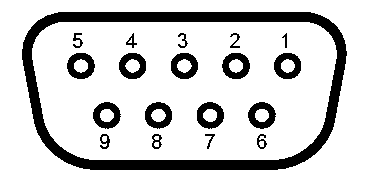
\includegraphics[width=1\textwidth]{grafiken/Numbered_DE9_female_Diagram.pdf}\\
    Front view
  \end{minipage}
  \hfill
  \begin{minipage}[b]{0.49\textwidth}
    \centering
    \begin{tabular}{cc}
      \toprule
      \textbf{Pin} & \textbf{Function} \\
      \toprule
      1 & Phase B1 \\ \midrule
      2 & Phase B2\\ \midrule
      3 & Phase A2 \\ \midrule
      4 & Phase A1 \\ \midrule
      5 & Ground \\ \midrule
      6 & +5V \\ \midrule
      7 & Sens 1 \\ \midrule
      8 & Sens 2 \\ \midrule
      9 & Sens 3 \\ \midrule
      Shield & NC \\
      \bottomrule
    \end{tabular}
  \end{minipage}
\caption[Pinout of the motor connectors.]{Pinout of the motor connectors.}
\label{pin_out}
\end{figure}

The power connector is a R7B female connector. Please refer to figure~\ref{pin_out_power} for its pinout.

\begin{figure}[h]
\begin{center}
\begin{minipage}[h]{0.49\textwidth}
    \centering
    %R7B female connector\\
    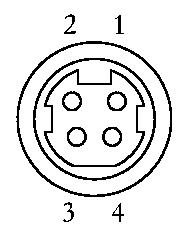
\includegraphics[width=0.55\textwidth]{grafiken/R7B.pdf}\\
    Front view
  \end{minipage}
  \hfill
  \begin{minipage}[h]{0.49\textwidth}
    \centering
    \begin{tabular}{cc}
      \toprule
      \textbf{Pin} & \textbf{Function} \\
      \toprule
      1 & + 24V \\ \midrule
      2 & Ground\\ \midrule
      3 & Ground \\ \midrule
      4 & + 24V  \\ \midrule
      Shield & NC \\
      \bottomrule
    \end{tabular}
  \end{minipage}
\end{center}
\caption[Pinout of the power connector.]{Pinout of the power connector.}
\label{pin_out_power}
\end{figure}






%\newpage

\clearpage


%\newpage
\printindex

% to get an empty page
%\newpage\null
%\thispagestyle{empty}
%\newpage

\end{document}















